\section{補遺}
\subsection{ネットワーク構造のパラメータ値の決め方}
\label{sec:Sparam}
ニューロンのネットワーク構造をsmall world networkによって表すために,初期次数と張り替え確率を実データから決める.
今回はこの値はニューロンのコネクションの割合と相互のコネクションの割合から決める.
興奮性ニューロン同士の6.7\%であり,そのうち双方向のコネクションの割合は24\%である\cite{Jouhanneau2015}.
発達中マウスの興奮性ニューロンから抑制性ニューロンへのコネクティビティと抑制性ニューロンから興奮性ニューロンへのコネクティビティはどちらも78\%であった\cite{Holmgren2003}.
成熟したマウスではより少ないと思われるが,データが見つからなかったため,40\%とした.
相互のコネクションの割合がランダムにエッジを作るよりも高いのは,近いニューロンにコネクションが作られやすいからだと考えられる.
これらのデータを実現するように初期次数と張り替え確率を調整した.
用いたパラメータを\Tabref{tab:parameter1}に示す.
抑制性ニューロン同士のコネクティビティは分からないため,興奮性ニューロンと同じにしている.

\begin{table}[htb]
  \center
  \begin{tabular}{|c|cc|} \hline
    結合の種類 & 初期次数 & 張り替え確率 \\ \hline
		同種類のニューロン間 & $0.0335 N$ & $0.3$ \\
		興奮性ニューロンと抑制性ニューロン間 & $0.2N$ & $0.3$\\ \hline
  \end{tabular}
  \caption{ネットワーク構造のパラメータ値}
  \label{tab:parameter1}
\end{table}

実際のネットワーク構造の作り方を説明する.
ネットワーク構造は興奮性ニューロン同士の結合,抑制性ニューロン同士の結合,興奮性ニューロンと抑制性ニューロン間の結合の3つに分けて作成する.
まず,全ニューロンのうち抑制性ニューロンと興奮性ニューロンのインデックスを決めておく.
全てのニューロンについて\Tabref{tab:parameter1}に従ってネットワークを作成し,それぞれに対応する隣接行列の上三角または下三角行列を取り出して結合する.
作成したいのは向きのある有向グラフなので,上三角行列と下三角行列を分けて作成する.

\subsection{スパイクシミュレーションの設定}
\label{sec:spikeparam}
スパイクシミュレーションで設定しなければならないのは,個々のニューロンの特徴パラメータ,重み付きのネットワーク構造,外部からのランダムな入力である.
これらについて説明する.

まず,個々のニューロンの特徴パラメータについて説明する.
このモデルではニューロンごとに4つのパラメータを設定する必要があり,そのパラメータでニューロンを特徴づける.
本論文では興奮性ニューロンにはregular spiking neurons,抑制性ニューロンにはfast spiking neuronsを用いる.
それらのパラメータを~\Tabref{tab:parameter2}に示す.
ただし,$r_e$と$r_i$は0から1の一様分布に従う確率変数である.

\begin{table}[htb]
  \center
  \begin{tabular}{|c|cccc|} \hline
    ニューロンの種類 & a & b & c & d \\ \hline
    興奮性ニューロン & 0.02 & 0.2 & $-65 + 15 r_e^2$ & $8 - 6r_e^2$ \\
    抑制性ニューロン & $0.02 + 0.08r_i$ & $0.25 - 0.05 r_i$ & -65 & 2 \\ \hline
  \end{tabular}
  \caption{Izhikevichモデルのパラメータ値}
  \label{tab:parameter2}
\end{table}

次に,重み付きのネットワーク構造$W \in \mathbb{R}^{N \times N}$について説明する.
ニューロン$i$から$j$へ結合があった場合,$w_{ij}$はニューロン$i$が発火した時にニューロン$j$の膜電位をどれだけ上昇させるかという数値である.
$W$は,前節で作成した$S$の非ゼロ要素を数値で置き換えることで作成する.
重み付きネットワーク構造$W$の作成方法は2種類ある:
\begin{enumerate}
  \item 全ての重みを同じ分布から生成する
  \item 同じグループへの興奮性ニューロンからの入力は強めにする
\end{enumerate}
1番目の方法では,興奮性ニューロンからの結合は標準偏差$\sigma_w = 1.5$の対数正規分布の$10$以下の分布,抑制性ニューロンからの結合は一様分布$U(-10,0)$からサンプルする.
\begin{align}
	w_{ij} = \begin{cases}
		\{\frac{1}{\sqrt{2 \pi \sigma_w^2}w} \exp \{ - \frac{(\ln w)^2}{2 \sigma_w^2}\} | w \in [0,10]\} & (s_{ij} = 1 \text{,$i$は興奮性ニューロン}) \\
		U(-10,0) & (s_{ij} = 1 \text{,$i$は抑制性ニューロン}) \\
		0 & (s_{ij} = 0)
  \end{cases}
	\label{eq:W}
\end{align}

2番目の方法では,同じグループの興奮性ニューロンからの結合は一様分布$U(7,10)$,異なるグループの興奮性ニューロンからの結合は標準偏差$\sigma_w = 1.5$の対数正規分布の$7$以下の分布,抑制性ニューロンからの結合は一様分布$U(-10,0)$からサンプルする.
対数正規分布を用いる理由は\cite{Song}のデータに基づく.
\begin{align}
	w_{ij} = \begin{cases}
		U(7,10) & (s_{ij} = 1 \text{,$i$は興奮性ニューロン,$i$と$j$は同じグループ}) \\
		\{\frac{1}{\sqrt{2 \pi \sigma_w^2}w} \exp \{ - \frac{(\ln w)^2}{2 \sigma_w^2} \} | w \in [0,7]\} & (s_{ij} = 1 \text{,$i$は興奮性ニューロン,$i$と$j$は異なるグループ}) \\
		U(-10,0) & (s_{ij} = 1 \text{,$i$は抑制性ニューロン}) \\
		0 & (s_{ij} = 0)
  \end{cases}
	\label{eq:W}
\end{align}

最後に外部からのランダムな入力について説明する.
ニューロンには観測範囲外からの入力がある(以降,外部入力とする).
そのため,シミュレーション中も外部からの電位を乱数としてニューロンの電位に足す.
本論文では,ニューロンの活動も外部入力の大きさで表現する.
活動していない興奮性ニューロンと抑制性ニューロンにはそれぞれ,$\mathcal{N}(0,9)$と$\mathcal{N}(0,0.01)$に従う乱数を足す.
活動している興奮性ニューロンと抑制性ニューロンの外部入力は,それぞれの正規分布の平均を$Ne_{plus}$と$Ni_{plus}$とする.
これらを\Tabref{tab:parameter3}に示す.
活動していないニューロンへの外部入力は\cite{Izhikevich2003}で用いられていたものを採用した.
ただし,興奮性ニューロンの活動時の外部入力は変化させた実験もある.

\begin{table}[htb]
  \center
  \begin{tabular}{|c|cc|} \hline
    ニューロンの種類 & 活動時の外部入力 & 活動していない時の外部入力 \\ \hline
		興奮性ニューロン & $\mathcal{N}(Ne_{plus},9)$ & $\mathcal{N}(0, 9)$ \\
		抑制性ニューロン & $\mathcal{N}(Ni_{plus}, 0.01)$ & $\mathcal{N}(0, 0.01)$ \\ \hline
  \end{tabular}
  \caption{シミュレーションに用いる外部入力の値}
  \label{tab:parameter3}
\end{table}

実際の脳でもこのように外部からの入力によってニューロンの活動を制御していると考えられる.
あるニューロングループを活動させる別の方法として,そのグループのハブとなるニューロンにのみ強い外部入力を与える方法も考えられる.

実際のマウスのニューロンの発火頻度を\cite{Watson2016}を元に\Tabref{tab:spike-frequency}に示す.
\Tabref{tab:art_dat}のnon-active120データの興奮性ニューロンと抑制性ニューロンの発火頻度を\Figref{fig:ex_frequency}と\Figref{fig:in_frequency}に示す.
実際のデータと人工データでオーダーは合っていることがわかる.
\Tabref{tab:spike-frequency}のデータは電気生理のデータなので,スパイク頻度の高いニューロンが観測される.
そのため,多少数値が異なっていてもオーダーが合っていれば良いと思われる.
\begin{table}[htb]
  \center
  \begin{tabular}{|c|ccc|} \hline
    ニューロンの種類 & 覚醒時(Hz) & ノンレム睡眠時(Hz) & レム睡眠時(Hz) \\ \hline
		興奮性ニューロン & $0.76 \pm 1.53$ & $0.69 \pm 0.86$ & $0.88 \pm 1.33$ \\
		抑制性ニューロン & $5.59 \pm 7.25$ & $4.69 \pm 5.62$ & $4.25 \pm 9.43$ \\ \hline
  \end{tabular}
  \caption{ニューロンごとの発火頻度の中央値}
  \label{tab:spike-frequency}
\end{table}
\begin{figure}[htbp]
    \begin{minipage}{0.5\hsize}
			\begin{center}
					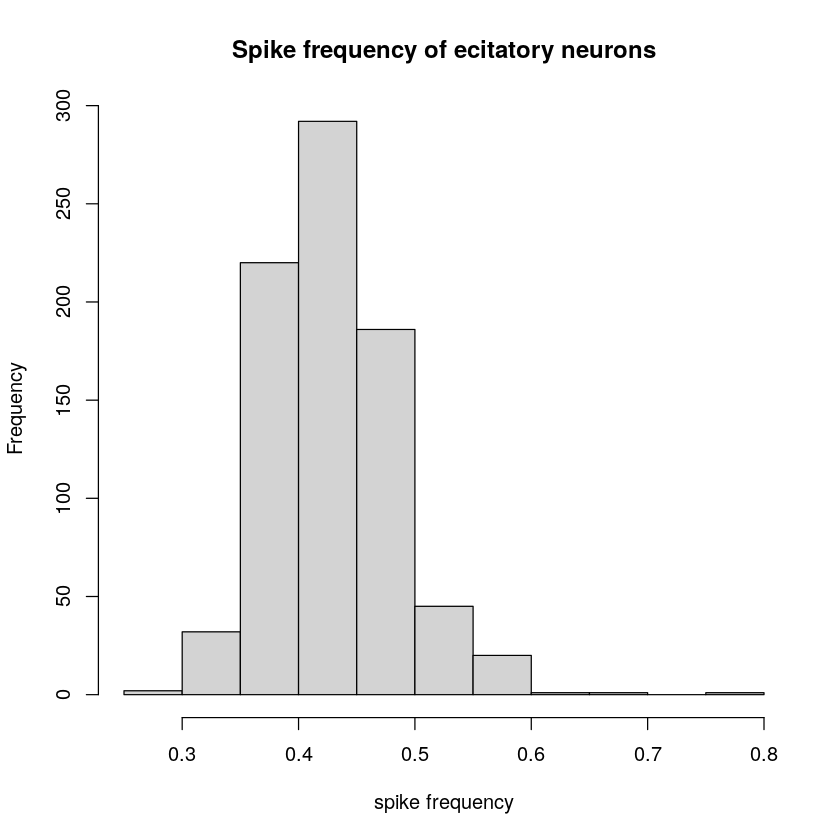
\includegraphics[width=\hsize]{ex_frequency}
					\caption{興奮性ニューロンのスパイク頻度のヒストラグム.}
					\label{fig:ex_frequency}
			\end{center}
		\end{minipage}
    \begin{minipage}{0.5\hsize}
			\begin{center}
					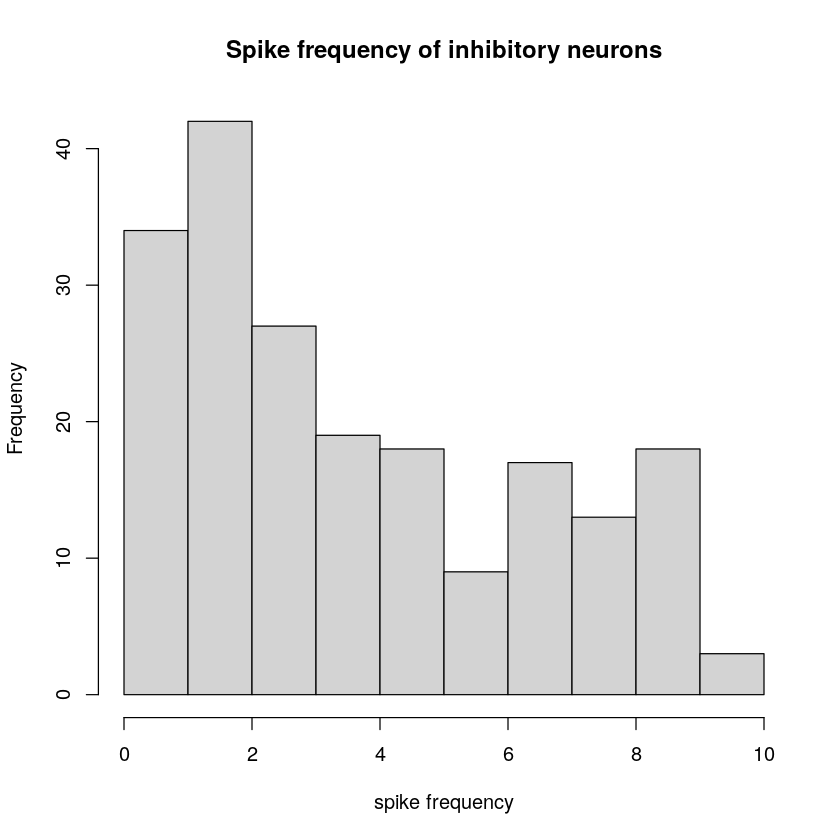
\includegraphics[width=\hsize]{in_frequency}
					\caption{抑制性ニューロンのスパイク頻度のヒストラグム.}
					\label{fig:in_frequency}
			\end{center}
		\end{minipage}
\end{figure}
